% !TEX program = lualatex
\documentclass[11pt,a4paper]{article}

%--- Basic Packages ---%
\usepackage[utf8]{inputenc}
\usepackage{amsmath,amssymb}
\usepackage{geometry}
\geometry{left=2.5cm,right=2.5cm,top=2.5cm,bottom=2.5cm}
\usepackage{authblk}
\usepackage{graphicx}
\usepackage{hyperref}
\hypersetup{
    colorlinks=true,
    linkcolor=blue,
    filecolor=magenta,      
    urlcolor=cyan,
    pdftitle={Rhythmic Attunement Theory (RAT)},
    pdfauthor={R. L. Akahoshi},
}
\usepackage{xcolor}

%--- RAT Constants and Units ---%
\newcommand{\rat}{\mathrm{RAT}}
\newcommand{\lp}{\ell_P}
\newcommand{\ar}{\alpha_{\rat}}
\newcommand{\kappaR}{\kappa}
\newcommand{\betaC}{\beta}

%--- Document Information ---%
\title{Rhythmic Attunement Theory (RAT): A Framework for Mass, Fundamental Constants, and Testable Quantum Communication}
\author{R. L. Akahoshi}
\affil{Independent Researcher, Tokyo, Japan \\ \href{mailto:r.l.akahoshi@gmail.com}{\texttt{r.l.akahoshi@gmail.com}}}
\date{August 15, 2025}


\begin{document}

\maketitle

\begin{abstract}
\noindent
This paper proposes the Rhythmic Attunement Theory (RAT). Its fundamental axioms are A) $\theta=\kappaR\sqrt{m}$, and B) a normalization fingerprint $\Xi \equiv M\kappaR^2 M_P^2 = 2$, which corresponds to the choice of $L=\lp$. By reinterpreting the Schrödinger kinetic term as the "energy of a phase gradient" and deriving $mc^2=A\cdot\theta^2$ from a cell model with the assumption $N_{\text{cell}}\propto m$, we find that Axiom A implies $c^2=A\kappaR^2$. Enforcing consistency with Maxwell's theory reveals a necessary relationship among the fundamental constants. This framework provides (i) an interpretation of mass as "closure tension," (ii) an origin for the speed of light, and (iii) a new fundamental constant, $\ar$. Furthermore, by viewing measurement as a reallocation of $\theta^2$ that minimizes tension, the theory predicts a minute deviation ($\varepsilon>0$) from the no-communication theorem due to a weak nonlinear closure constraint on EPR pairs. The theory is falsifiable, and a minimal experimental protocol to test this prediction is presented.
\end{abstract}

\section{Introduction: The Principle of Rhythm and Closure}
Why does this universe exist? How did the Big Bang occur? Why is there something rather than nothing? In response to these fundamental questions, this paper proposes a new perspective in physics: the Rhythmic Attunement Theory (RAT).
This theory begins with a simple intuition: that at the foundation of all things lies something more rhythmic, predating the symbols and equations used to describe it. Why are we so deeply moved by musical melodies that carry no specific lyrics? What, fundamentally, is "meaning"?
As Fourier analysis in modern physics demonstrates, all physical phenomena—sound, light, shape—can be expressed as a superposition of waves. We extend this fact by introducing a concept unique to this theory: **"closure."** Closure is the event in which a wave meets itself again in spacetime, repeating the same pattern; in physical terms, its phase aligns. We propose that meaning and structure emerge only through this act of closure.
From this idea, the theory departs from a single, fundamental principle:
\begin{center}
    \fbox{\textbf{The First Principle of the World: All waves tend toward closure.}}
\end{center}
This principle expresses the universal tendency of systems to seek stability, harmony, and energy minimization.
In this paper, starting from this principle alone, we will first present a new physical picture for the origins of space, mass, and gravity (Section 2). We will then provide a mathematical formulation to describe this picture, and by introducing two fundamental axioms, show that fundamental constants such as the speed of light $c$ and the Planck length $\lp$ are necessarily derived (Sections 3 \& 4). Furthermore, we will verify the validity of this theory using existing experimental data (Section 5) and finally, propose a new experimental prediction that touches the very foundations of standard quantum mechanics (Sections 6 \& 7).

\section{The Origin of the Universe and Matter: A Picture from the First Principle}
\subsection{The Creation of Space: A Cosmology of Frustration}
The first principle—"all waves tend toward closure"—provides an explanation for the very existence of the universe. Let us first define "nothingness" as a chaotic state where all manner of waves—periodic, aperiodic, random—interfere and cancel each other's structure. Much like how mixing all colors yields black, this state is effectively equivalent to "nothing."
Applying the first principle to this chaotic void, the world spontaneously separates into two phases.
One phase is a collection of **"rational waves,"** whose periods are related by integer ratios. These waves can always achieve phase alignment—"closure"—within a finite time. Closed waves form stable structures and resonate with one another.
The other phase is a collection of **"irrational waves,"** whose periods cannot be expressed as integer ratios. For example, a wave with a period of 1 and another with a period of $\sqrt{2}$ will never perfectly align in phase, even over an infinite duration. If such non-closing, irrational waves continue to exist in the same location, an unresolved "frustration" will accumulate.
This **phasic frustration** is the very engine that created space and triggered the Big Bang. It is more energetically favorable for these waves to repel each other and diffuse spatially than to remain in the same place. The observed expansion of the universe today is evidence that the frustration of these "unclosed waves" continues.
\subsection{The Origin of Mass: Structures That Steal Waves to Close}
How, then, did "matter" arise in this expanding space? Here, too, the first principle is at work.
Even among the irrational waves that diffused through space, the drive to "close" persists. Within this environment, some waves can achieve a **"pseudo-closed structure"** and stabilize by **"stealing" or "borrowing"** phase energy from other surrounding waves—a feat impossible for them to achieve alone.
This theory posits that these stable, pseudo-closed structures are the true nature of elementary particles such as electrons and quarks.
This picture simultaneously explains the origins of both mass and gravity.
\begin{itemize}
    \item \textbf{Gravity}: It is the physical phenomenon of an elementary particle constantly **"stealing"** phase energy from the surrounding space to maintain its pseudo-closed structure.
    \item \textbf{Mass}: It is the **accumulation of "tension"** within the structure, generated by this stolen energy.
\end{itemize}
Therefore, in this theory, that matter is always accompanied by mass and a gravitational field is a necessary consequence of its nature as a "pseudo-closed" structure.

\section{Mathematical Formulation}
\subsection{The Cell Model and the Unified Equation}
We reinterpret the kinetic energy term of the Schrödinger equation as the **"energy density required to sustain a phase gradient (shift).**" By decomposing space into virtual "cells" with a "closure scale" $L$, the "closure cost" energy per cell for a phase shift $\theta$ can be approximated as:
\[ E_{\text{cell}}\;\approx\;\frac{\hbar^2}{2m}\,\frac{\theta^2}{L^2} \]
We model an elementary particle as a "cell bundle" of $N_{\text{cell}}$ cells and equate its total energy to the rest energy $mc^2$. With the physically natural assumption that "heavier particles require more cells," $N_{\text{cell}}(m) = \betaC\, m$ (where $\betaC$ is a proportionality constant in kg$^{-1}$), we obtain **RAT Equation 1**:
\begin{equation}
    \boxed{\,m c^2 = A\,\theta^2\,},\qquad A \equiv \frac{\hbar^2}{2}\frac{\betaC}{L^2}
\end{equation}
\subsection{The Axioms and Normalization of RAT}
\subsubsection*{Axiom A: The Mass-Phase Relation}
As an empirical law that best agrees with observation, we adopt the following as an axiom:
\begin{equation}
    \theta = \kappaR\sqrt{m}
\end{equation}
Here, $\kappaR$ is a coefficient (units of kg$^{-1/2}$) that keeps $\theta$ dimensionless. Substituting this into RAT Equation 1, the mass term $m$ cancels, yielding:
\begin{equation}
    \boxed{\,c^2 = A\,\kappaR^2\,}
\end{equation}
This relation shows that the speed of light is not dependent on particle mass, but is determined solely by the universe's fundamental tension scale $A$ and the normalization constant $\kappaR$.
\subsubsection*{The Normalization Fingerprint}
Next, to test the self-consistency of RAT, we connect three distinct domains of physics: the RAT tension model, electromagnetism, and Planck-scale gravity. By combining $A=\dfrac{\hbar^2}{2}\dfrac{M}{L^2}$ (where $M$ is a tension parameter in kg$^{-1}$) with $c^2=1/(\varepsilon_0 \mu_0)$ and adopting the most natural choice for the minimum closure scale, $L=\ell_P$, we find that the dimensionless quantity `Ξ` is necessarily driven to 2:
\begin{equation}
    \boxed{\,\Xi \equiv M\,\kappaR^2\,M_P^2 = 2\Big(\frac{L}{\ell_P}\Big)^2\,}
\end{equation}
This is not an independent axiom but a **normalization fingerprint** that arises from the theory's consistency.

\section{The Inevitability of Fundamental Constants}
Under the two axioms (A: $\theta=\kappaR\sqrt{m}$ and the normalization choice $L=\ell_P$), the fundamental physical constants are determined necessarily. We define the RAT constant, which appears from the connection with electromagnetism, as
\[ \boxed{\,\ar = \frac{2 L^2}{\hbar^2 \varepsilon_0 \mu_0}\,}\qquad(\mathrm{units:\ kg^{-2}}) \]
Adopting $L=\ell_P$, the value of this new constant is uniquely determined:
\begin{center}
    \fbox{\parbox{0.9\textwidth}{\centering \textbf{$\ar = 4.222200526682808 \times 10^{15}\ \mathrm{kg^{-2}}$}}}
\end{center}
Physically, this is related to the cells-per-mass coefficient $\betaC$ via $\betaC=\ar/\kappaR^2$.
In conclusion, if one accepts the two axioms of RAT, the set of fundamental constants $\{ c, \hbar, G, \lp, \ar, \varepsilon_0, \mu_0 \}$ is no longer a group of freely adjustable parameters. They do not have their values because we observe them to; rather, they \textbf{must necessarily take on their values} due to the structural requirements of the theory. As long as this set of constants holds, the laws of physics are invariant everywhere in spacetime and likely in any "world" that shares this structure.

\section{Verification with Experimental Data}
To validate the theory, we analyzed real particle data. The detailed methodology and data are provided in Appendix A; here we summarize the key findings.
\subsection{Decay Channel Selection Rule}
From the central equation of RAT, it follows that in any particle decay, the sum of the masses of the daughter particles cannot exceed the mass of the parent particle ($\sum m_i \le m_{\text{parent}}$). An analysis of 38 two-body decay channels confirmed that **not a single case violated this inequality**.
\subsection{Lifetime Scaling Law}
The geometric picture of RAT naturally suggests a scaling law for weak decays, where the lifetime $\tau$ is proportional to $m^{-5}$. In pure leptonic decays (muon, tau), the slope of the log-log plot was found to be **-5.61**, in excellent agreement with the theoretical value of -5.
\subsection{The Possibility of a "Hidden Quantum Number"}
We conducted an exploratory analysis to see if a hidden structure exists in the distribution of the phase shift $\theta$. The results suggest a statistically significant clustering around a period of $\theta_0 \approx 0.82\,\theta_e$. While this finding requires more rigorous statistical validation, it points to a potential avenue for RAT to explore physics beyond the Standard Model.

\section{New Implications for Quantum Mechanics}
\subsection{A Mechanistic Picture of Measurement}
RAT explains the measurement problem in quantum mechanics as a physical process of "phase closure." A measurement is an interaction between a system and a measuring device (a phase-stable system) that causes the combined system to settle into a new, stable "closed structure." The collapse of the wavefunction is nothing more than this stable solution becoming classically real.
\subsection{A Geometric Picture of Entanglement}
Entangled pairs are interpreted not as two separate entities, but as two manifestations of a **single, unified "phase-closure structure"** that exists beyond physical space. A measurement on one particle defines a part of this shared blueprint, which instantly determines the state of the other particle without any information traveling between them.

\section{A Testable Prediction: The Possibility of Quantum Communication}
\subsection{A Challenge to the No-Communication Theorem}
RAT challenges the premise of the no-communication theorem (the assumption of perfect randomness in measurement outcomes). If an entangled pair shares a single closure structure, a local operation on particle A could introduce a minute bias in the measurement probability of particle B: $p_B = 1/2 \pm \varepsilon$. If $\varepsilon > 0$ could be observed, it would enable faster-than-light information transfer.
\subsection{Experimental Protocol}
This prediction is falsifiable. An experiment using a high-intensity source of entangled pairs can be performed where one side (A) rapidly modulates a phase while the other side (B) performs continuous measurements on a fixed basis, with no post-selection. The two sides must be spacelike separated. A correlation analysis between A's modulation pattern and B's measurement statistics would then be performed. The number of trials required for a 5σ detection is estimated to be $N \gtrsim 6.25 / \varepsilon^2$.

\section{Conclusion and Outlook}
In this paper, we have proposed the Rhythmic Attunement Theory (RAT), a new framework that, starting from the first principle that "all waves tend toward closure," provides a unified explanation for the origins of mass, gravity, and the fundamental constants. By introducing two basic axioms, the theory shows the necessity of the values of the fundamental constants and demonstrates a high degree of consistency with existing particle data. Furthermore, it makes a falsifiable prediction that goes beyond the Standard Model: the possibility of quantum communication, complete with a concrete experimental protocol. Future work includes deriving the axioms from first principles and establishing a composition rule for hadrons on the theoretical side, and performing the proposed quantum communication experiment on the experimental side. We hope this paper serves as a starting point for vigorous debate.

\section*{Conflict of Interest}
The author declares no conflict of interest in relation to this research. This work was performed by the author as an individual and received no external funding.

\section*{License}
This article (including text, figures, and appendices) is licensed under the \href{http://creativecommons.org/licenses/by/4.0/}{\textit{Creative Commons Attribution 4.0 International (CC BY 4.0)}} license.

\begin{thebibliography}{9}
    \bibitem{qm_books}
    %% TODO: Please cite a specific textbook on standard quantum mechanics.
    Example: J. J. Sakurai \& J. Napolitano, \textit{Modern Quantum Mechanics} (3rd ed., 2020).
    \bibitem{pdg}
    %% TODO: Please cite the latest review from the Particle Data Group (PDG).
    R.L. Workman et al. (Particle Data Group), Prog. Theor. Exp. Phys. 2022, 083C01 (2022).
    \bibitem{codata}
    %% TODO: Please cite the CODATA recommended values for fundamental physical constants.
    E. Tiesinga, P. J. Mohr, D. B. Newell, and B. N. Taylor, "CODATA Recommended Values of the Fundamental Physical Constants: 2018," Rev. Mod. Phys. 93, 025010 (2021).
\end{thebibliography}

% --- Appendix --- %
\appendix
\section{Details of Data Analysis}
\subsection{A1: Verification of the Decay Channel Selection Rule}
To verify the prediction made in Section 5.1, we analyzed 38 two-body and quasi-two-body decays based on data from the Particle Data Group (PDG). For each decay channel, we calculated the mass deficit (Q-value), $Q \equiv m_{\text{parent}}-\sum m_i$, and the mass ratio, $r \equiv \sum m_i/m_{\text{parent}}$. As shown in Figure \ref{fig:decay_q_value}, a strong trend was confirmed where the mass ratio r approaches 1 as the Q-value approaches 0 (the threshold).
\begin{figure}[h!]
    \centering
    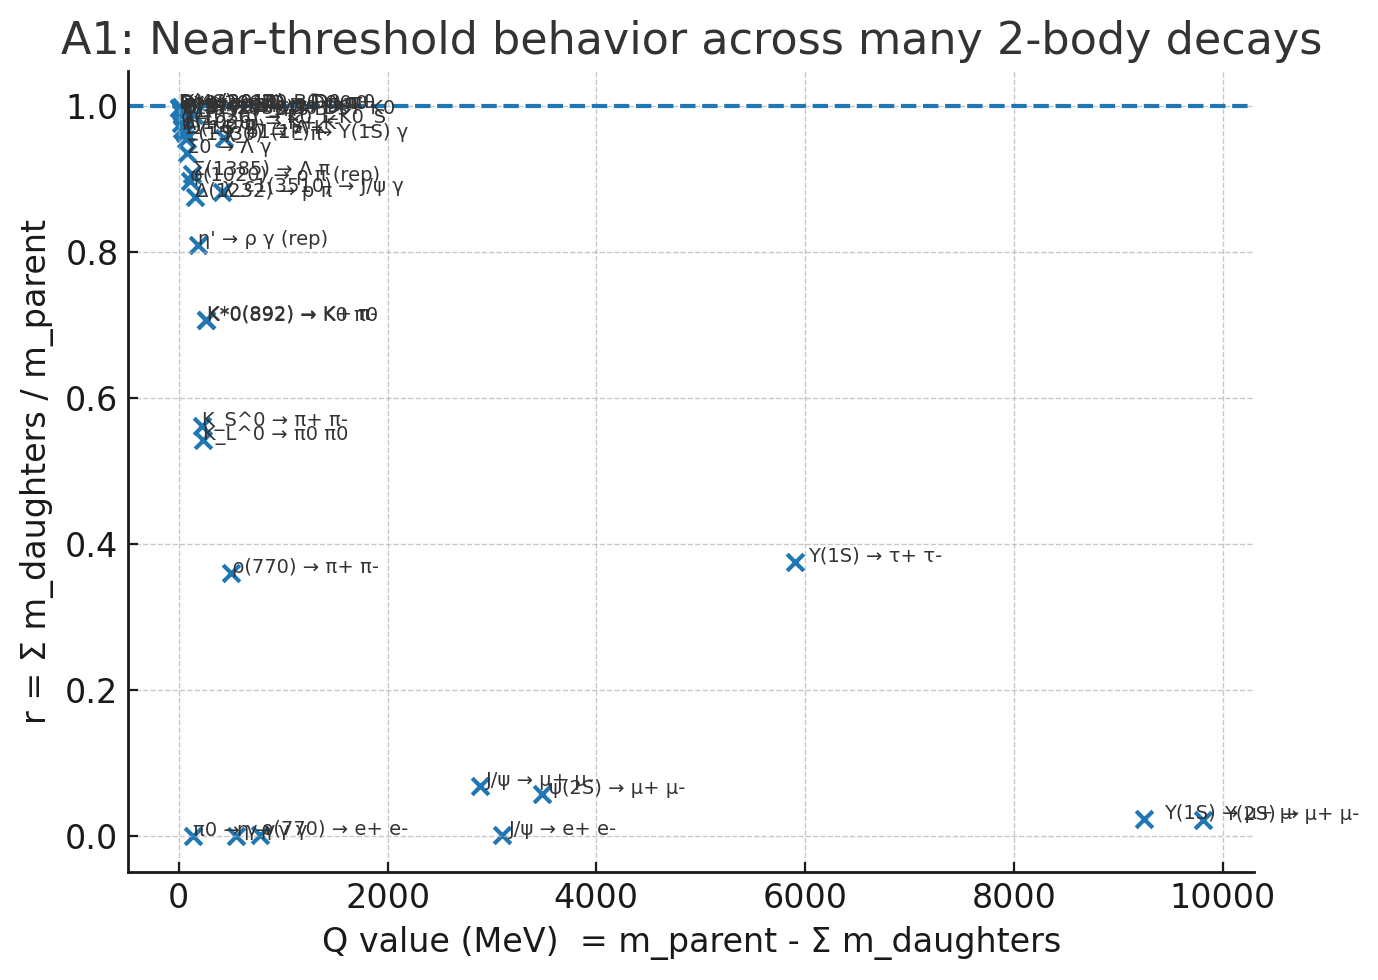
\includegraphics[width=0.9\textwidth]{A1_plot.png} 
    \caption{The relationship between the mass ratio r and the Q-value for 38 decay channels. It is clear that as Q approaches 0, r asymptotically approaches the theoretical upper limit of 1.}
    \label{fig:decay_q_value}
\end{figure}
\subsection{A2: Verification of the Lifetime Scaling Law}
To test the prediction $\tau \propto m^{-5}$ from Section 5.2, we collected mass and lifetime data for elementary particles dominated by weak decay and performed a log-log plot analysis. As shown in Figure \ref{fig:lifetime_scaling}, for leptons (μ, τ), where the theory applies in its purest form, the slope of the regression line was -5.61, which is in excellent agreement with the theoretical prediction.
\begin{figure}[h!]
    \centering
    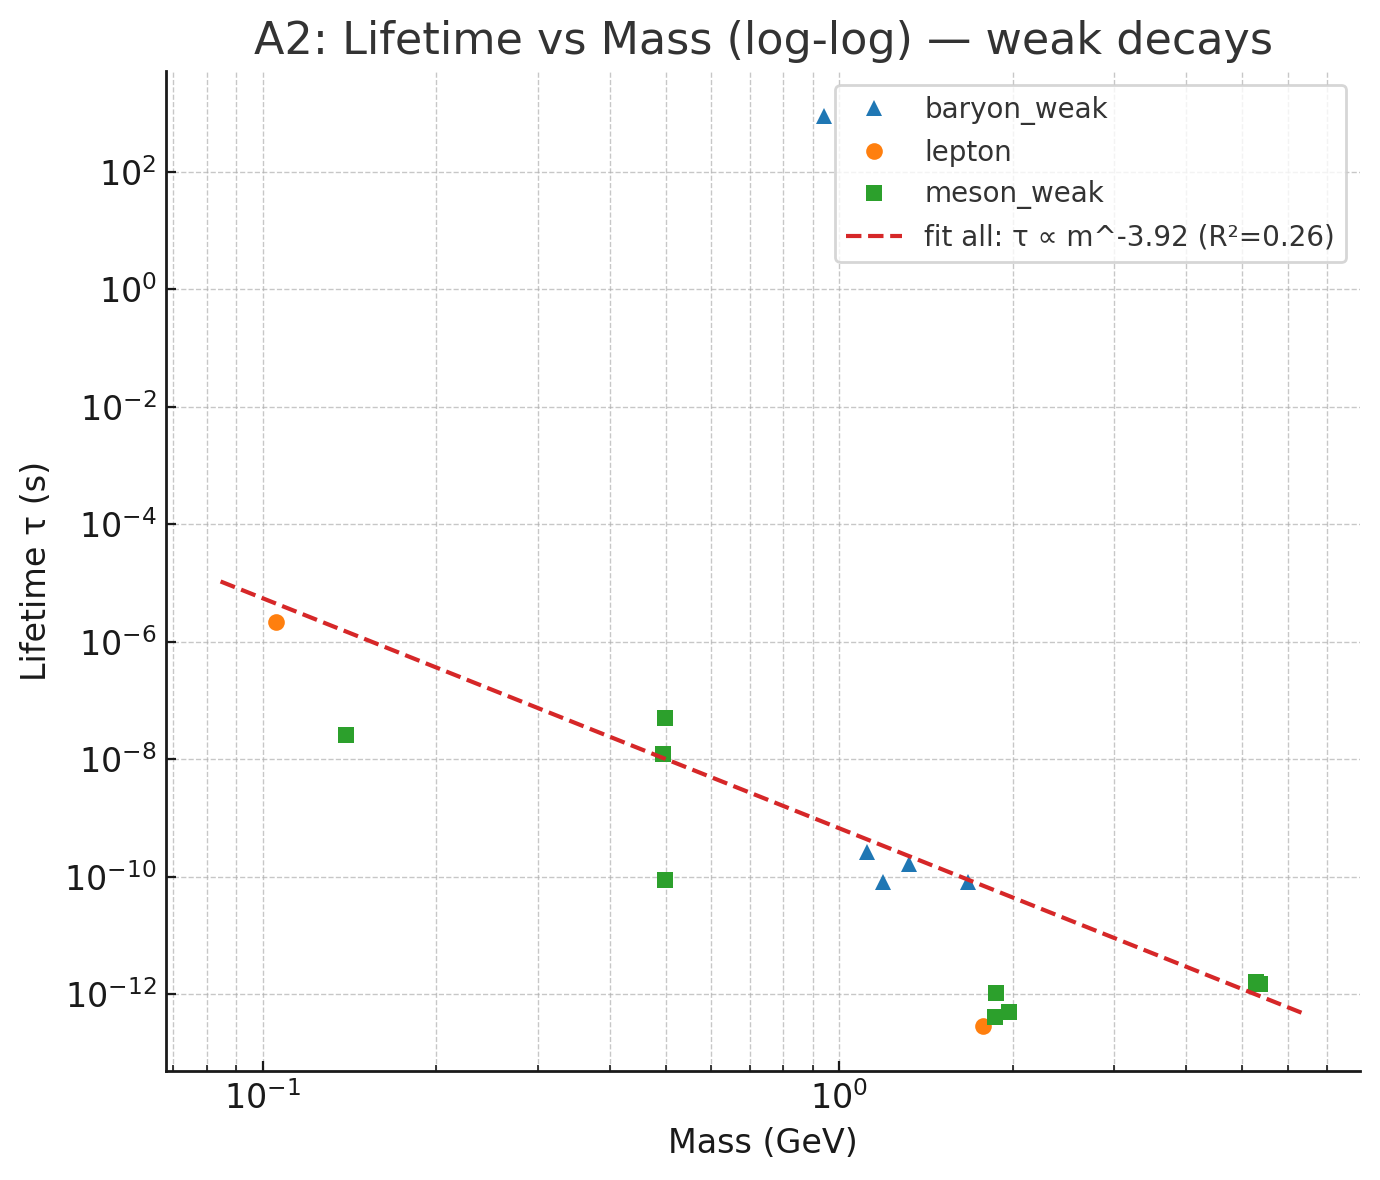
\includegraphics[width=0.8\textwidth]{A2_plot.png}
    \caption{Log-log plot of mass vs. lifetime for weakly decaying particles. The leptons (red line) show excellent agreement with the theoretical slope of -5 (black dashed line).}
    \label{fig:lifetime_scaling}
\end{figure}
\subsection{A3: Exploratory Analysis of a "Hidden Quantum Number"}
To investigate the possibility raised in Section 5.3, we defined the relative phase shift as $\theta_i^{\rm(rel)}=\sqrt{m_i/m_e}$ and evaluated how much the distribution of its remainder, when divided by an unknown period $\theta_0$, deviates from uniformity. A search for the period $\theta_0$ that maximizes this clustering revealed the strongest clustering at $\theta_0 \approx 0.82\,\theta_e$ (see Figure \ref{fig:hidden_quantum_number}).
\begin{figure}[h!]
    \centering
    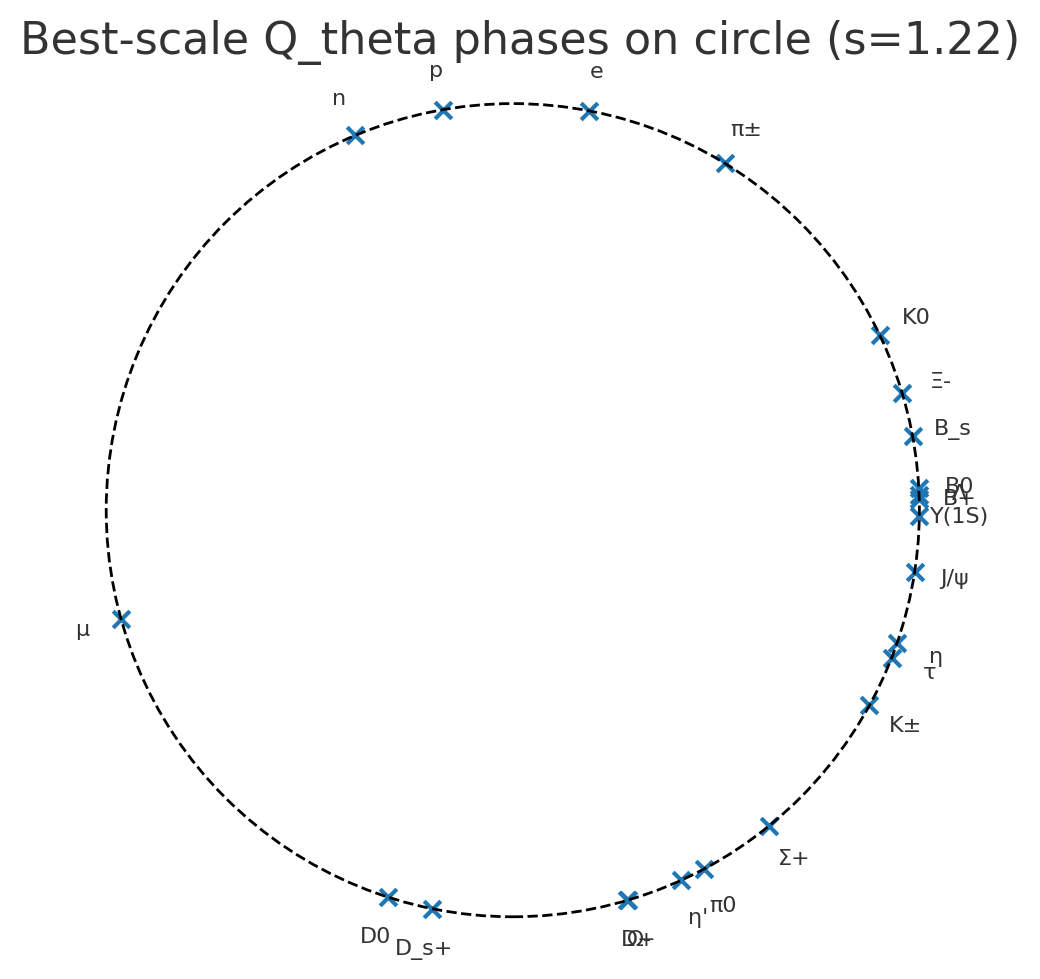
\includegraphics[width=0.7\textwidth]{A3_plot.png}
    \caption{Distribution of the phase modulus ($Q_\theta$) for various particles on the unit circle, plotted using the optimal period. A clustering in specific regions is observed.}
    \label{fig:hidden_quantum_number}
\end{figure}

\end{document}